% #############################################################################
% This is Chapter 3
% !TEX root = ../main.tex
% #############################################################################
% Change the Name of the Chapter i the following line
\fancychapter{State of the Art}
\cleardoublepage
This thesis leverages state-of-the-art technologies, many of which are under active development or about to be released. The focus is on creating a software program utilizing vector databases, \ac{LLM}, and \ac{RAG}, all of which are evolving at a rapid pace. These fields offer a mix of open-source libraries and paid solutions, providing flexibility in implementation. While this section highlights libraries most relevant to the thesis, it acknowledges the possibility of their obsolescence by the time this draft is finalized.

\section{Vector Databases, testing}
Why is vector database important for this project?
Vector databases are database specifically designed to store vectors and retrieve them. Since in the project with have a RAG pipeline that generates embeddings of documents, which are a vector representation of text. The embedding vectors must be stored and retrieved efficiently, even at great scale. \ac{VD} offer features such as vector indexing that enable fast retrieval at a large scale. Vector Databases prove to be the most prominent method for storage of the embeddings and enabling fast scalable semantic search.
How is it used?


Why is it better than other implementations?
What is required to run this database?
Weaviate \cite{weaviate} is an open-source vector database designed to store both objects and vectors, enabling the combination of vector search with structured filtering. It integrates seamlessly with various machine learning models, allowing for efficient data storage and retrieval. Weaviate offers a range of features, including built-in vector and hybrid search, advanced filtering, and out-of-the-box \ac{RAG} capabilities. It supports integrations with multiple model providers, such as Cohere, Hugging Face, and OpenAI, enhancing its flexibility and adaptability to specific needs. Developers can interact with Weaviate using client libraries available in Python, JavaScript/TypeScript, Go, and Java, facilitating ease of use across different programming environments. Additionally, Weaviate can be deployed fully locally, providing options for self-hosted setups. Its cloud-native architecture ensures scalability, fault tolerance, and security, making it suitable for both prototyping and production at scale.

\section{Vector Databases}
\label{sec:vector-databases}

\subsection{Motivation and Importance}
Vector databases (\ac{VD}) are specialized systems designed to store and retrieve high-dimensional vector representations of data, also known as embeddings. In the context of this project, where a Retrieval-Augmented Generation (\ac{RAG}) pipeline is employed, embeddings of documents are generated to numerically encode their semantic content. Efficient storage and retrieval of these embeddings is essential, particularly when operating at scale. Traditional relational or document-based databases are not optimized for similarity-based retrieval; instead, vector databases employ dedicated indexing and search strategies to enable fast, scalable, and semantically meaningful queries.

\subsection{Core Concepts}

\hspace*{1em} \textbf{Vector Embeddings.}  
Embeddings transform unstructured data (e.g., text, images, or audio) into numerical vectors that capture semantic relationships. Similar objects are placed closer together in the vector space. For example, the terms \emph{dog} and \emph{wolf} would be embedded near each other, while \emph{banana} would appear in a distant region of the space (see Fig.~\ref{fig:vector-embedding}).  

\begin{figure}[h]
    \centering
    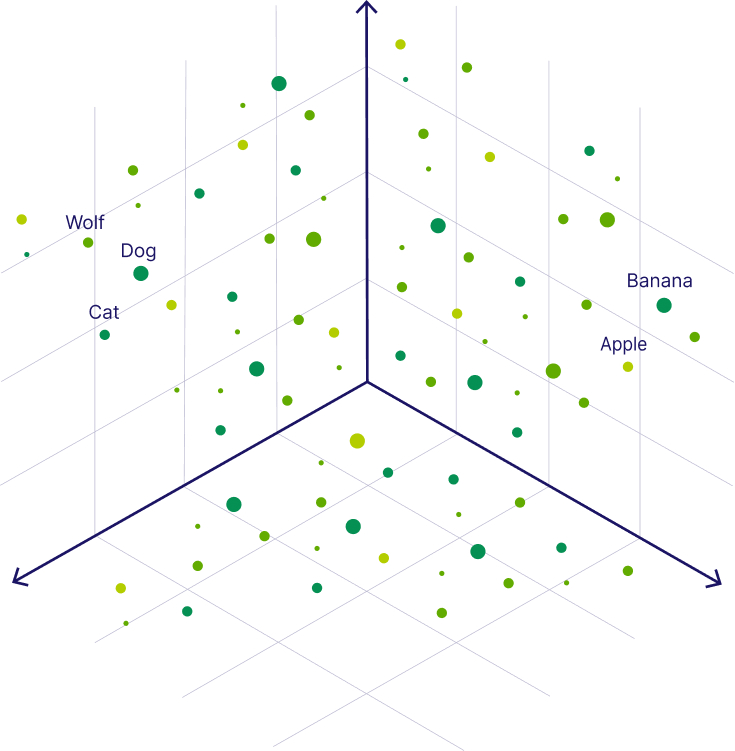
\includegraphics[width=0.55\linewidth]{Images/vector-embedding.jpg}
    \caption{Example of vector embeddings where semantically related terms are placed closer in the vector space}
    \label{fig:vector-embedding}
\end{figure}

\textbf{Vector Search.}  
Vector search (also known as similarity search or semantic search) allows retrieval of items by computing the distance between embeddings. Queries are converted into vectors and matched against the database to find the nearest neighbors (see Fig.~\ref{fig:vector-search}). Unlike keyword search, which relies on lexical matches, vector search captures contextual meaning, producing more human-like and relevant results.

\begin{figure}[h]
    \centering
    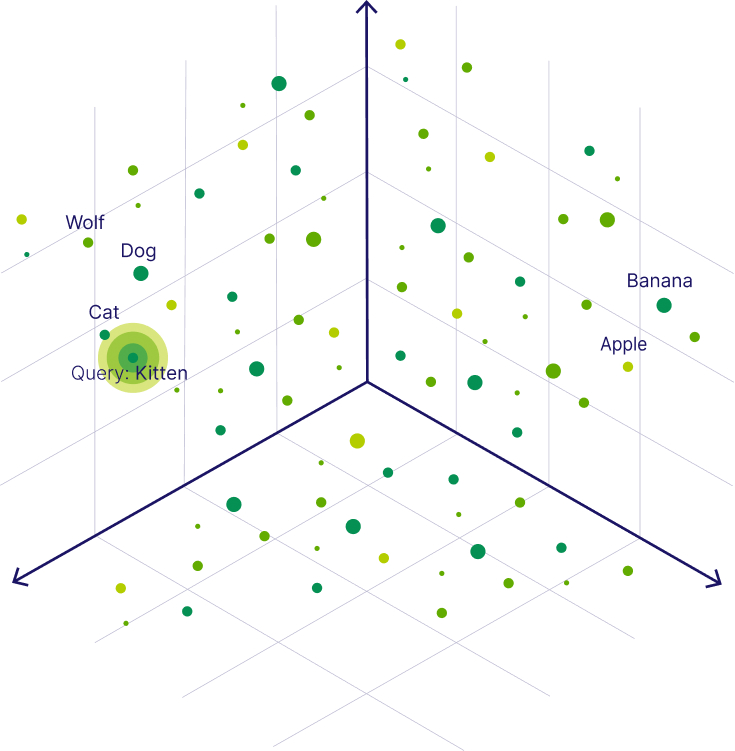
\includegraphics[width=0.55\linewidth]{Images/vector-search.jpg}
    \caption{Illustration of semantic search: the query vector ``kitten'' retrieves nearest neighbors such as ``cat''.}
    \label{fig:vector-search}
\end{figure}

\textbf{Vector Indexing.}  
To enable efficient retrieval in high-dimensional spaces, vector databases use approximate nearest neighbor (\ac{ANN}) algorithms such as Hierarchical Navigable Small World (\ac{HNSW}) graphs, product quantization, or locality-sensitive hashing. These indexing techniques drastically reduce search time, even for millions or billions of vectors, without significant loss of accuracy.

\subsection{Advantages over Other Approaches}
Compared to traditional relational databases or full-text search engines (e.g., BM25-based systems), vector databases offer several advantages:
\begin{itemize}
    \item \textbf{Semantic retrieval:} captures meaning beyond exact keyword matches.
    \item \textbf{Scalability:} optimized for billions of vectors while maintaining low-latency search.
    \item \textbf{Flexibility:} supports multimodal embeddings (text, images, audio).
    \item \textbf{Hybrid search:} many systems (e.g., Weaviate, Pinecone, Milvus) combine symbolic (keyword) and vector search, enabling richer query capabilities.
\end{itemize}

\subsection{Requirements}
Running a vector database requires:
\begin{itemize}
    \item \textbf{Compute resources:} CPU or GPU acceleration for index building and similarity search.
    \item \textbf{Memory and storage:} sufficient RAM to host vector indexes and SSD-based storage for persistence.
    \item \textbf{Integration with embedding models:} embeddings must be generated consistently using the same model to ensure vectors reside in the same semantic space.
    \item \textbf{Indexing strategy:} selection of ANN algorithm based on use-case tradeoffs between accuracy, speed, and memory consumption.
\end{itemize}

\subsection{Relevance for this Project}
In this thesis, the \ac{VD} is a fundamental component of the RAG pipeline. It ensures that document embeddings can be efficiently stored, indexed, and retrieved to support semantic search across large-scale and heterogeneous datasets. This infrastructure enables the system to deliver accurate, contextually relevant results in near real-time, which is critical for enterprise information retrieval.


\section{Optical Character Recognition Engines}
\label{sec:ocr}
Optical Character Recognition (OCR) engines are essential tools for converting textual information from various formats, such as PDFs or images, into machine-readable text. These engines operate through a series of steps that involve image preprocessing, character segmentation, and text recognition. 
Character recognition is achieved using machine learning models and heuristic functions. The process involves the following key techniques. Feature Extraction to identify characters based on their visual features, such as shapes, lines, and pixel patterns. Pattern Matching to compare characters against predefined patterns or templates stored within the \ac{OCR} engine. Contextual Analysis, leveraging information about the language of the document to improve predictions and accurately interpret words within the language's grammar.
\begin{itemize}
    \item Nougat\cite{blecher2023nougatneuralopticalunderstanding}: Known for its high accuracy in text extraction, especially from complex documents. It excels at converting text into Markdown format, preserving the document's structure.
    \item Tesseract: An open-source engine that supports over 100 languages, including Portuguese. However, its performance may be less reliable for languages other than English or for documents with complex layouts.
    \item Google Vision API: : A cloud-based tool offering advanced OCR capabilities. It employs well-trained Convolutional Neural Networks (CNNs) to identify characters with high precision, making it one of the most accurate solutions available.
\end{itemize}

\section{Large Language Models (LLMs)}
\ac{LLM}s are a cornerstone of modern \ac{NLP}. These models can be accessed or installed through platforms like Hugging Face, which provides a comprehensive repository of pre-trained models. With continuous improvements in training methodologies, larger datasets, and more advanced architectures, \ac{LLM}s ARE Becoming increasingly effective and efficient at understanding and generating natural language.
These advancements bring significant benefits to the program being developed in this project, particularly in two key areas:
\begin{itemize}
    \item Vector Embeddings: \ac{LLM}s can generate high-quality vector embeddings from textual data, capturing deeper semantic relationships that enhance information retrieval
    \item Summarization: \ac{LLM}s can summarize documents and large text blocks, providing a more accurate representation of the user context and improving the clarity of the retrieved information.
\end{itemize}
This thesis focuses on understanding and analyzing the architectures (e.g., Transformer-based models like GPT, BERT, and LLaMA) and the training techniques of \ac{LLM}s. A comprehensive analysis will be conducted to evaluate why a specific \ac{LLM} is best suited for the project's requirements.

The continuous evolution of \ac{LLM}s ensures that new models will offer even better results, further enhancing the performance and capabilities of this project. By leveraging state-of-the-art \ac{LLM}s, this program aims to deliver an improved user experience through better indexing and summarization of documents.

\section{Sentence Transformers}
Sentence Transformers are BERT-based encoder models designed to generate dense vector representations (embeddings) of entire sentences or passages. 
They were introduced in 2019 \cite{reimers2019sentencebertsentenceembeddingsusing} as an adaptation of the BERT architecture, which was originally built for token-level classification tasks.

With the use of Siamese and Triplet network structures on top of BERT, SBERT modifies the architecture to operate at the sentence level. Instead of encoding a pair of sentences jointly, as in the cross-encoder setup of standard BERT, SBERT processes each sentence independently with a shared BERT encoder. This produces fixed-size embeddings that can later be compared directly using cosine similarity or other distance metrics, making large-scale similarity search computationally feasible.

In a Siamese setup, two identical BERT encoders with shared weights process different input sentences. Their embeddings are then compared, allowing the network to learn similarity or classification objectives. This design ensures that semantically similar sentences are mapped to nearby points in the embedding space, while dissimilar ones are pushed apart.

Triplet networks extend this idea by processing three inputs simultaneously: an anchor sentence, a positive sentence with similar meaning, and a negative sentence with unrelated meaning. The model is trained to minimize the distance between the anchor and the positive embedding, while maximizing the distance between the anchor and the negative embedding. This objective directly enforces a semantically meaningful structure in the embedding space, making the representations more robust for tasks such as \ac{STS} and information retrieval.

Since BERT outputs contextual embeddings for individual tokens, an additional pooling layer is required to derive a single sentence vector, as shown in Figure~\ref{fig:Sentence_embedding}. In \cite{reimers2019sentencebertsentenceembeddingsusing}, the preferred pooling method for \ac{STS} tasks is mean pooling, which turns multiple token embeddings into a single sentence embedding.\footnote{Other pooling strategies, such as using the \texttt{[CLS]} token or max pooling, were also evaluated but performed worse for semantic similarity tasks.}

\begin{figure}[h!]
    \centering
    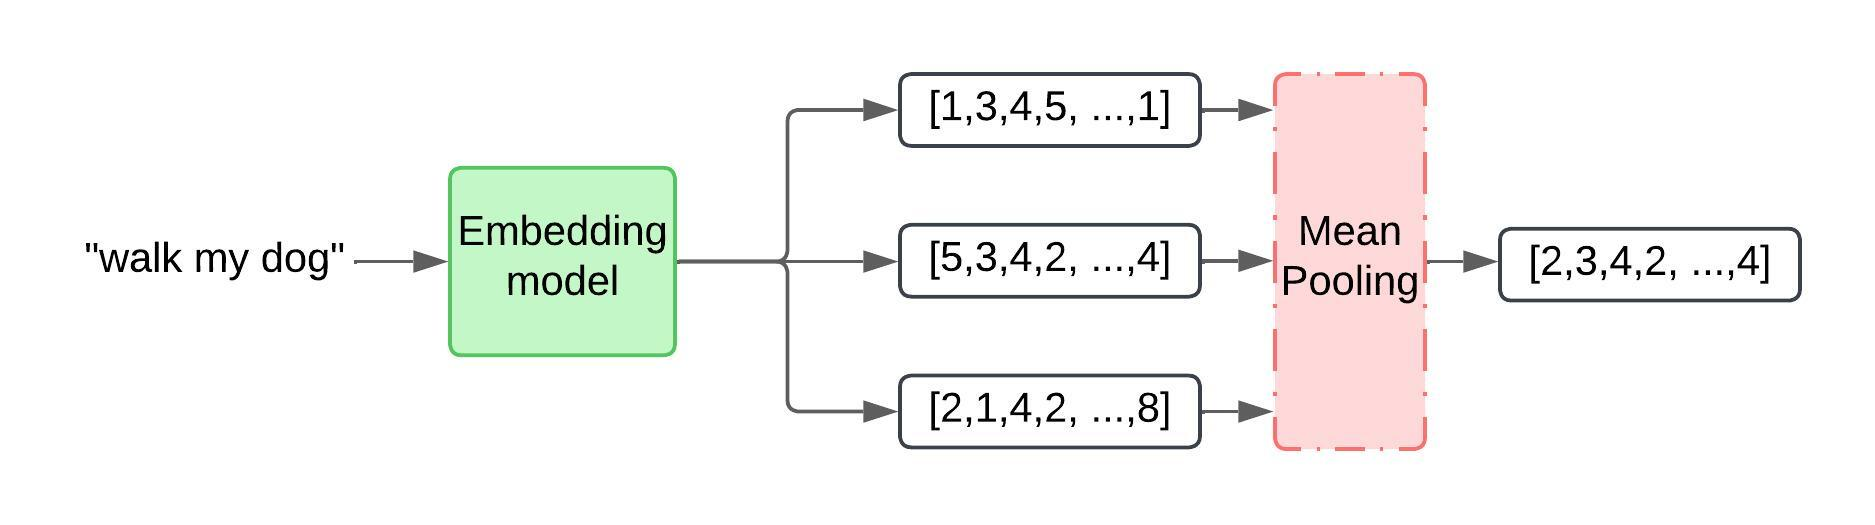
\includegraphics[width=1\linewidth]{Figures/Sentence_Embedding.jpeg}
    \caption{Simplified illustration of sentence embedding through mean pooling.}
    \label{fig:Sentence_embedding}
\end{figure}

To ensure that these embeddings capture sentence-level meaning, SBERT is fine-tuned on tasks such as Natural Language Inference (NLI), Semantic Textual Similarity (STS), and triplet training. 

When trained on NLI data with a classification objective, SBERT further compares pairs of sentence embeddings by constructing a combined feature vector $(u, v, |u-v|)$, where $u$ and $v$ are the pooled embeddings of the two sentences. This representation proved effective in downstream tasks such as the Semantic Textual Similarity benchmark (STS-b).

The quality of a Sentence Transformer is ultimately reflected in the accuracy and robustness of the embeddings it produces. Recent research has extended these methods to Portuguese, with the current state-of-the-art being the \textit{Serafim 900M IR} model \cite{gomes2024opensentenceembeddingsportuguese}, which has been specifically trained and benchmarked for \ac{STS} and \ac{IR} tasks.


\section{Text Similarity metrics}
Since this thesis aims to enhance semantic search through Retrieval-Augmented Generation (\ac{RAG}), 
evaluating similarity between texts becomes a critical component for evaluating the model and methodology. 
No single metric fully captures the notion of similarity: some emphasize exact lexical overlap, 
while others account for structural variation or semantic equivalence. 
Therefore, a diverse set of metrics is employed to provide a more comprehensive assessment, 
ensuring that evaluation reflects the multifaceted nature of semantic search.

\begin{table}[H]
\centering
\caption{Evaluation metrics and their relevance to semantic search in RAG pipelines.}
\begin{tabular}{|p{3cm}|p{5cm}|p{7cm}|}
\hline
\textbf{Metric} & \textbf{What it Measures} & \textbf{Relevance to RAG} \\
\hline
Exact Match & Binary check for identical prediction and reference & Strict baseline for correctness; detects precise retrieval or generation \\
\hline
Substring Match & Whether the reference occurs as a contiguous substring of the output & Useful for cases where the gold answer is included verbatim in a longer generated passage \\
\hline
Token Recall & Proportion of reference tokens covered by the output & Captures coverage of essential information; valuable when retrieving partial fragments of long documents \\
\hline
Jaccard Similarity \cite{jaccard1901distribution} & Lexical overlap between token sets, ignoring frequency and order & Evaluates vocabulary similarity between retrieved/generated output and reference \\
\hline
Levenshtein Similarity \cite{levenshtein1966binary} & Normalized edit distance over tokens (insertions, deletions, substitutions) & Sensitive to word order; highlights structural differences important for coherent retrieval \\
\hline
ROUGE-n (F1) \cite{lin2004rouge} & n-gram overlap (unigrams for ROUGE-1, bigrams for ROUGE-2) & Balances precision and recall of content; checks both coverage and local phrase structure \\
\hline
BERT Cosine Similarity \cite{reimers2019sentence} & Semantic closeness of dense embeddings & Captures deep semantic equivalence, even under paraphrasing; most aligned with semantic search goals \\
\hline
Overlap Coefficient \cite{simpson1960similarity} & Intersection size normalized by the smaller token set & Rewards complete coverage of the reference, even if additional tokens are present \\
\hline
BLEU (sentence-level) \cite{papineni2002bleu} & n-gram precision with brevity penalty & Evaluates fluency and lexical faithfulness; checks whether generated answers resemble the phrasing of references \\
\hline
\end{tabular}
\label{tab:metrics}
\end{table}

By combining these metrics, the evaluation captures complementary perspectives:  
lexical accuracy (Exact Match, Substring, Jaccard), structural similarity (Levenshtein, ROUGE, BLEU), coverage of reference information (Token Recall, Overlap coefficient), and semantic equivalence (BERT cosine).This multidimensional evaluation approach allows for a comprehensive assessment by testing both surface-level metrics and deeper semantic understanding.

\section{Advanced RAG with Reasoning, Context awareness}

\section{LLM Profiling}